\iffalse
This file is protected by Copyright. Please refer to the COPYRIGHT file
distributed with this source distribution.

This file is part of OpenCPI <http://www.opencpi.org>

OpenCPI is free software: you can redistribute it and/or modify it under the
terms of the GNU Lesser General Public License as published by the Free Software
Foundation, either version 3 of the License, or (at your option) any later
version.

OpenCPI is distributed in the hope that it will be useful, but WITHOUT ANY
WARRANTY; without even the implied warranty of MERCHANTABILITY or FITNESS FOR A
PARTICULAR PURPOSE. See the GNU Lesser General Public License for more details.

You should have received a copy of the GNU Lesser General Public License along
with this program. If not, see <http://www.gnu.org/licenses/>.
\fi

%----------------------------------------------------------------------------------------
% Update the docTitle and docVersion per document
%----------------------------------------------------------------------------------------
\def\docTitle{OpenCPI\\ Rx App Guide\\ (E310 Supplement)}
\def\docVersion{1.4}
%----------------------------------------------------------------------------------------
\documentclass{article}
\iffalse
This file is protected by Copyright. Please refer to the COPYRIGHT file
distributed with this source distribution.

This file is part of OpenCPI <http://www.opencpi.org>

OpenCPI is free software: you can redistribute it and/or modify it under the
terms of the GNU Lesser General Public License as published by the Free Software
Foundation, either version 3 of the License, or (at your option) any later
version.

OpenCPI is distributed in the hope that it will be useful, but WITHOUT ANY
WARRANTY; without even the implied warranty of MERCHANTABILITY or FITNESS FOR A
PARTICULAR PURPOSE. See the GNU Lesser General Public License for more details.

You should have received a copy of the GNU Lesser General Public License along
with this program. If not, see <http://www.gnu.org/licenses/>.
\fi
% Any changes to this document should be made in opencpi.git
\author{} % Force author to be blank
%----------------------------------------------------------------------------------------
% Paper size, orientation and margins
%----------------------------------------------------------------------------------------
\usepackage{geometry}
\geometry{
        letterpaper, % paper type
        portrait,    % text direction
        left=.75in,  % left margin
        top=.75in,   % top margin
        right=.75in, % right margin
        bottom=.75in % bottom margin
 }
%----------------------------------------------------------------------------------------
% Header/Footer
%----------------------------------------------------------------------------------------
\usepackage{fancyhdr} \pagestyle{fancy} % required for fancy headers
\renewcommand{\headrulewidth}{0.5pt}
\renewcommand{\footrulewidth}{0.5pt}
\rhead{\small{ANGRYVIPER Team}}
% \rfoot{\thepage}
%----------------------------------------------------------------------------------------
% Appendix packages
%----------------------------------------------------------------------------------------
\usepackage[toc,page]{appendix}
%----------------------------------------------------------------------------------------
% Defined Commands & Renamed Commands
%----------------------------------------------------------------------------------------
\renewcommand{\contentsname}{Table of Contents}
\renewcommand{\listfigurename}{List of Figures}
\renewcommand{\listtablename}{List of Tables}
\newcommand{\todo}[1]{\textcolor{red}{TODO: #1}\PackageWarning{TODO:}{#1}} % To do notes
\newcommand{\code}[1]{\texttt{#1}} % For inline code snippet or command line
%----------------------------------------------------------------------------------------
% Various packages
%----------------------------------------------------------------------------------------
\usepackage[usenames,dvipsnames]{xcolor} % for color names see https://en.wikibooks.org/wiki/LaTeX/Colors
\usepackage{hyperref}  % for linking urls and lists
\usepackage{graphicx}  % for including pictures by file
\usepackage{listings}  % for coding language styles
\usepackage{rotating}  % for sideways table
\usepackage{pifont}    % for sideways table
\usepackage{pdflscape} % for landscape view
\usepackage{subfig}
\hyphenation{ANGRY-VIPER} % Tell it where to hyphenate
\hyphenation{Cent-OS} % Tell it where to hyphenate
\hyphenation{install-ation} % Tell it where to hyphenate
\uchyph=0 % Never hyphenate acronyms like RCC (I think this overrides ANGRYVIPER above)
\renewcommand\_{\textunderscore\allowbreak} % Allow words to break/newline on underscores
%----------------------------------------------------------------------------------------
% Table packages
%----------------------------------------------------------------------------------------
\usepackage{longtable} % for long possibly multi-page tables
\usepackage{tabularx} % c=center,l=left,r=right,X=fill
% These define tabularx columns "C" and "R" to match "X" but center/right aligned
\newcolumntype{C}{>{\centering\arraybackslash}X}
\newcolumntype{R}{>{\raggedleft\arraybackslash}X}
\usepackage{float}
\floatstyle{plaintop}
\usepackage[tableposition=top]{caption}
\newcolumntype{P}[1]{>{\centering\arraybackslash}p{#1}}
\newcolumntype{M}[1]{>{\centering\arraybackslash}m{#1}}
%----------------------------------------------------------------------------------------
% Block Diagram / FSM Drawings
%----------------------------------------------------------------------------------------
\usepackage{tikz}
\usetikzlibrary{shapes,arrows,fit,positioning}
\usetikzlibrary{automata} % used for the fsm
%----------------------------------------------------------------------------------------
% Colors Used
%----------------------------------------------------------------------------------------
\usepackage{colortbl}
\definecolor{blue}{rgb}{.7,.8,.9}
\definecolor{ceruleanblue}{rgb}{0.16, 0.32, 0.75}
\definecolor{drkgreen}{rgb}{0,0.6,0}
\definecolor{deepmagenta}{rgb}{0.8, 0.0, 0.8}
\definecolor{cyan}{rgb}{0.0,0.6,0.6}
\definecolor{maroon}{rgb}{0.5,0,0}
%----------------------------------------------------------------------------------------
% VHDL Coding Language Style
% modified from: http://latex-community.org/forum/viewtopic.php?f=44&t=22076
%----------------------------------------------------------------------------------------
\lstdefinelanguage{VHDL}
{
        basicstyle=\ttfamily\footnotesize,
        columns=fullflexible,keepspaces,      % https://tex.stackexchange.com/a/46695/87531
        keywordstyle=\color{ceruleanblue},
        commentstyle=\color{drkgreen},
        morekeywords={
    library,use,all,entity,is,port,in,out,end,architecture,of,
    begin,and, signal, when, if, else, process, end,
        },
        morecomment=[l]--
}
%----------------------------------------------------------------------------------------
% XML Coding Language Style
% modified from: http://tex.stackexchange.com/questions/10255/xml-syntax-highlighting
%----------------------------------------------------------------------------------------
\lstdefinelanguage{XML}
{
        basicstyle=\ttfamily\footnotesize,
        columns=fullflexible,keepspaces,
        morestring=[s]{"}{"},
        morecomment=[s]{!--}{--},
        commentstyle=\color{drkgreen},
        moredelim=[s][\color{black}]{>}{<},
        moredelim=[s][\color{cyan}]{\ }{=},
        stringstyle=\color{maroon},
        identifierstyle=\color{ceruleanblue}
}
%----------------------------------------------------------------------------------------
% DIFF Coding Language Style
% modified from http://tex.stackexchange.com/questions/50176/highlighting-a-diff-file
%----------------------------------------------------------------------------------------
\lstdefinelanguage{diff}
{
        basicstyle=\ttfamily\footnotesize,
        columns=fullflexible,keepspaces,
        breaklines=true,                                % wrap text
        morecomment=[f][\color{ceruleanblue}]{@@},      % group identifier
        morecomment=[f][\color{red}]-,                  % deleted lines
        morecomment=[f][\color{drkgreen}]+,             % added lines
        morecomment=[f][\color{deepmagenta}]{---},      % Diff header lines (must appear after +,-)
        morecomment=[f][\color{deepmagenta}]{+++},
}
%----------------------------------------------------------------------------------------
% Python Coding Language Style
% modified from
%----------------------------------------------------------------------------------------
\lstdefinelanguage{python}
{
        basicstyle=\ttfamily\footnotesize,
        columns=fullflexible,keepspaces,
        keywordstyle=\color{ceruleanblue},
        commentstyle=\color{drkgreen},
        stringstyle=\color{orange},
        morekeywords={
    print, if, sys, len, from, import, as, open,close, def, main, for, else, write, read, range,
        },
        comment=[l]{\#}
}
%----------------------------------------------------------------------------------------
% Fontsize Notes in order from smallest to largest
%----------------------------------------------------------------------------------------
%    \tiny
%    \scriptsize
%    \footnotesize
%    \small
%    \normalsize
%    \large
%    \Large
%    \LARGE
%    \huge
%    \Huge

\date{Version \docVersion} % Force date to be blank and override date with version
\title{\docTitle}
\lhead{Rx App Guide}
%----------------------------------------------------------------------------------------
%\usepackage[T1]{fontenc} % http://tex.stackexchange.com/a/181119
\usepackage{graphicx}
\graphicspath{ {figures/} }
\usepackage{textcomp}

\begin{document}
\maketitle
%\thispagestyle{fancy}
\newpage
	\begin{center}
	\textit{\textbf{Revision History}}
		\begin{table}[H]
		\label{table:revisions} % Add "[H]" to force placement of table
			\begin{tabularx}{\textwidth}{|c|X|l|}
			\hline
			\rowcolor{blue}
			\textbf{Revision} & \textbf{Description of Change} & \textbf{Date} \\
			\hline
			v1.3.1-E3XX & Updated for E310 support & 3/2018 \\
			\hline
			v1.4 & Updated with simplications and references to assets' document & 9/2018 \\
			\hline
			\end{tabularx}
		\end{table}
	\end{center}

\newpage
\tableofcontents
\pagebreak
\vspace{1pc}
\hrule
\def\assetsdoc{\noindent For more information on this application, see \code{ocpi.assets}'s more in-depth version of the \textit{RX\_app} document.}
\section{Document Scope}
This document describes the ANGRYVIPER Receive demo application or ``Rx App". It includes a description of the RX App application and instructions on how to setup the various supported hardware platforms, build and execution of the application.

\section{Description}
\assetsdoc

\section{Hardware Portability}
This application is specific to the \verb+e3xx+ platform.

\section{Building the Application}
\subsection{Common Application Worker Dependencies}
The following application workers, sorted by component library name, must be built prior to building the RX application assembly. See Appendix A for the parameter configurations used in the application, and see the individual component datasheets for more information.\par\bigskip
	\begin{minipage}[t]{.5\textwidth}
	\begin{itemize}
		\item ocpi.core
			\subitem file\_write.rcc
		\item ocpi.assets.util\_comps
			\subitem timestamper.hdl
		\item ocpi.assets.dsp\_comps
			\subitem cic\_dec.hdl
			\subitem complex\_mixer.hdl
			\subitem iq\_imbalance\_fixer.hdl
			\subitem dc\_offset\_filter.hdl
	\end{itemize}
	\end{minipage}

\subsection{Hardware-Specific Worker Dependencies}
The following workers, sorted by component library name, must be built prior to building RX app. See Appendix A for the parameter configurations used in the application, and see the individual component datasheets for more information and build instructions.\par\bigskip
	\begin{minipage}[t]{\textwidth}
	\textbf{E310}
	\begin{itemize}
		\item ocpi.bsp.e310.cards
			\subitem e3xx\_mimo\_xcvr\_filter\_proxy.rcc
			\subitem e3xx\_mimo\_xcvr\_filter.hdl
			\subitem e3xx\_i2c.hdl
			\subitem e3xx\_rx.rcc
			\subitem e3xx\_mimo\_xcvr\_ad5662.hdl
	\end{itemize}
	\end{minipage} \medskip

\newpage

\subsection{HDL Assembly and HDL Container}
\assetsdoc
\begin{landscape}
\subsection{Performance and Resource Utilization}
\input{../../../hdl/assemblies/dc_offset_iq_imbalance_mixer_cic_dec_timestamper/utilization.inc}
\end{landscape}

\subsection{Executable}
\noindent To build for the E310 (which runs the xilinx13\_4 PetaLinux operating system), run the following command from the \textit{rx\_app} directory:\par\medskip
\texttt{ ocpidev build --rcc-platform xilinx13\_4 }\par\medskip
\assetsdoc
\section{Testing the Application}
\subsection{Sample Test Setup}
\assetsdoc
\subsection{Artifacts}
\assetsdoc \\
\noindent Appendix B includes a list of the artifacts required for each platform and mode.
\subsection{Arguments to executable}
\assetsdoc
\subsection{Library Path Requirements}
\noindent Prior to running the application, the environment variable OCPI\_LIBRARY\_PATH must be configure, such that, all of the Rx application's run-time artifacts can be located. OpenCPI conveniently provides access to a project's run-time artifacts at the top-level of each project in a directory called artifacts. Reference the OpenCPI Application Development Guide for more about OCPI\_LIBRARY\_PATH. \par\medskip

\noindent Run ``\code{make show}'' in the application directory for a recommended \code{OCPI\_LIBRARY\_PATH}.

\subsection{Expected results}
\noindent A python script is included with the application for plotting the received data in both the time and frequency domain. Using the test setup shown above and the default settings for the GNUradio block diagram, run the application with the following arguments:\par\medskip

\small

\noindent\textbf{E310}
\scriptsize
\noindent
\begin{verbatim}
# Usage is:
# ./target-xilinx13_4/rx_app rf_tune_freq data_bw rf_bw rf_gain bb_bw bb_gain if_tune_freq runtime enable_timestamps frontend
  ./target-xilinx13_4/rx_app 1000         0.512   -1    24      1     -1      0.256        1       1                 e3xx
\end{verbatim}
\small
\par\medskip
\noindent The output file can then be plotted with the python script with the following syntax and the output can be seen below:\par\medskip
\noindent\texttt{python ./scripts/plotAndFftAndTime.py odata/rx\_app\_raw.out complex 18000 256000 16352}\par
	\begin{figure}[h]
	 	\centering
		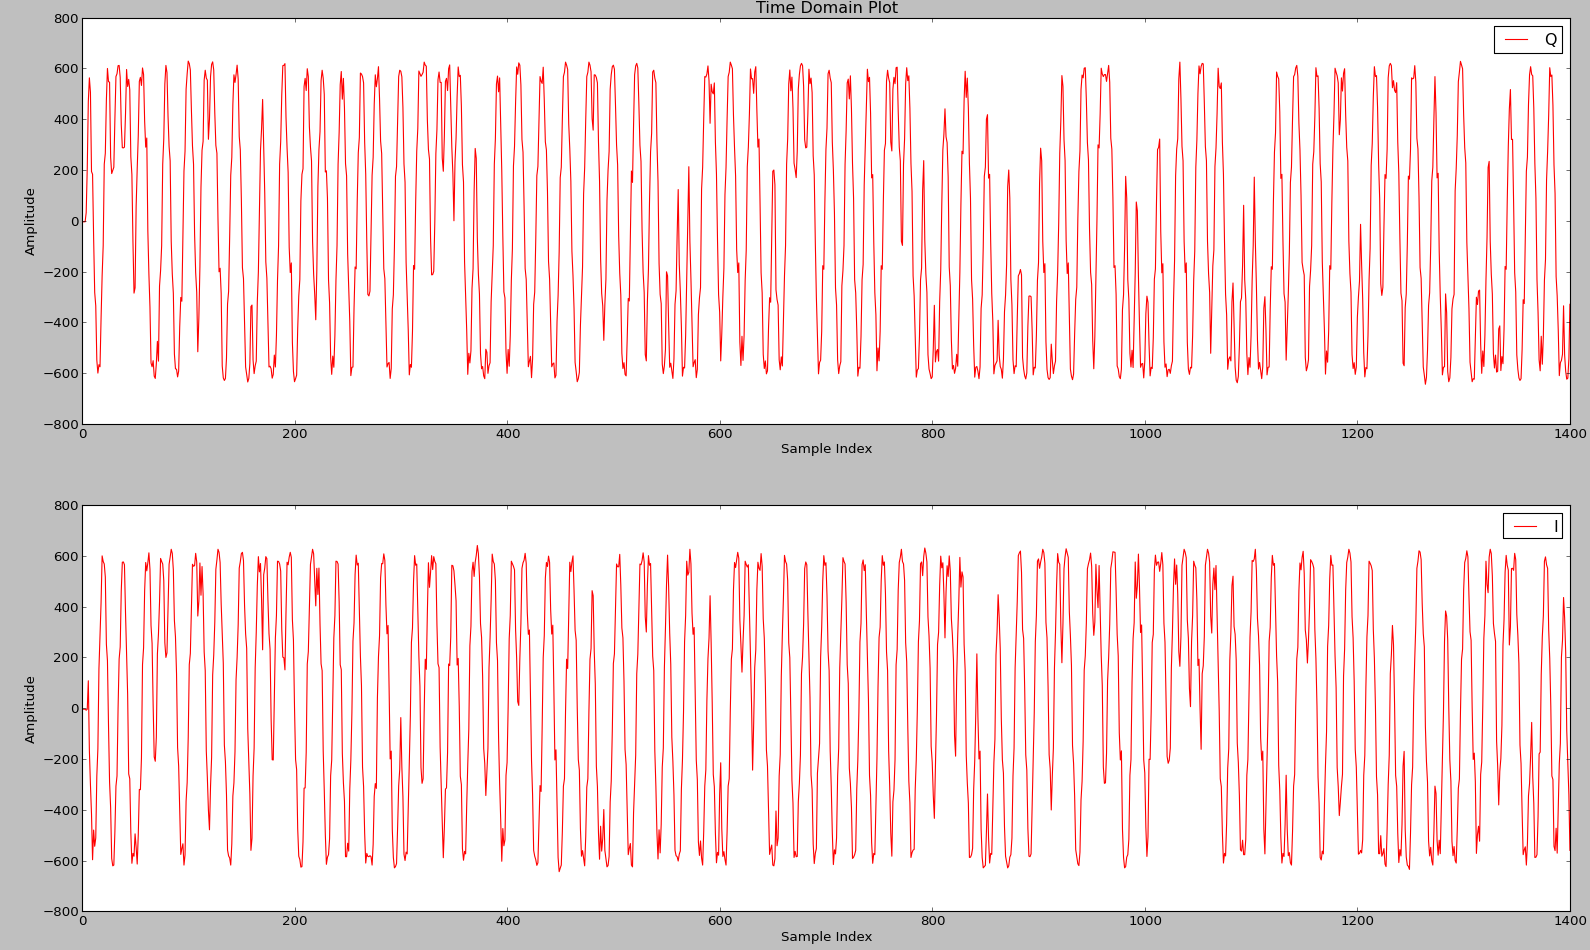
\includegraphics[scale=.2]{rx_app_iq_plot}
		\label{fig:rx_app_iq_plot}
	\end{figure}
	\begin{figure}[h]
	 	\centering
		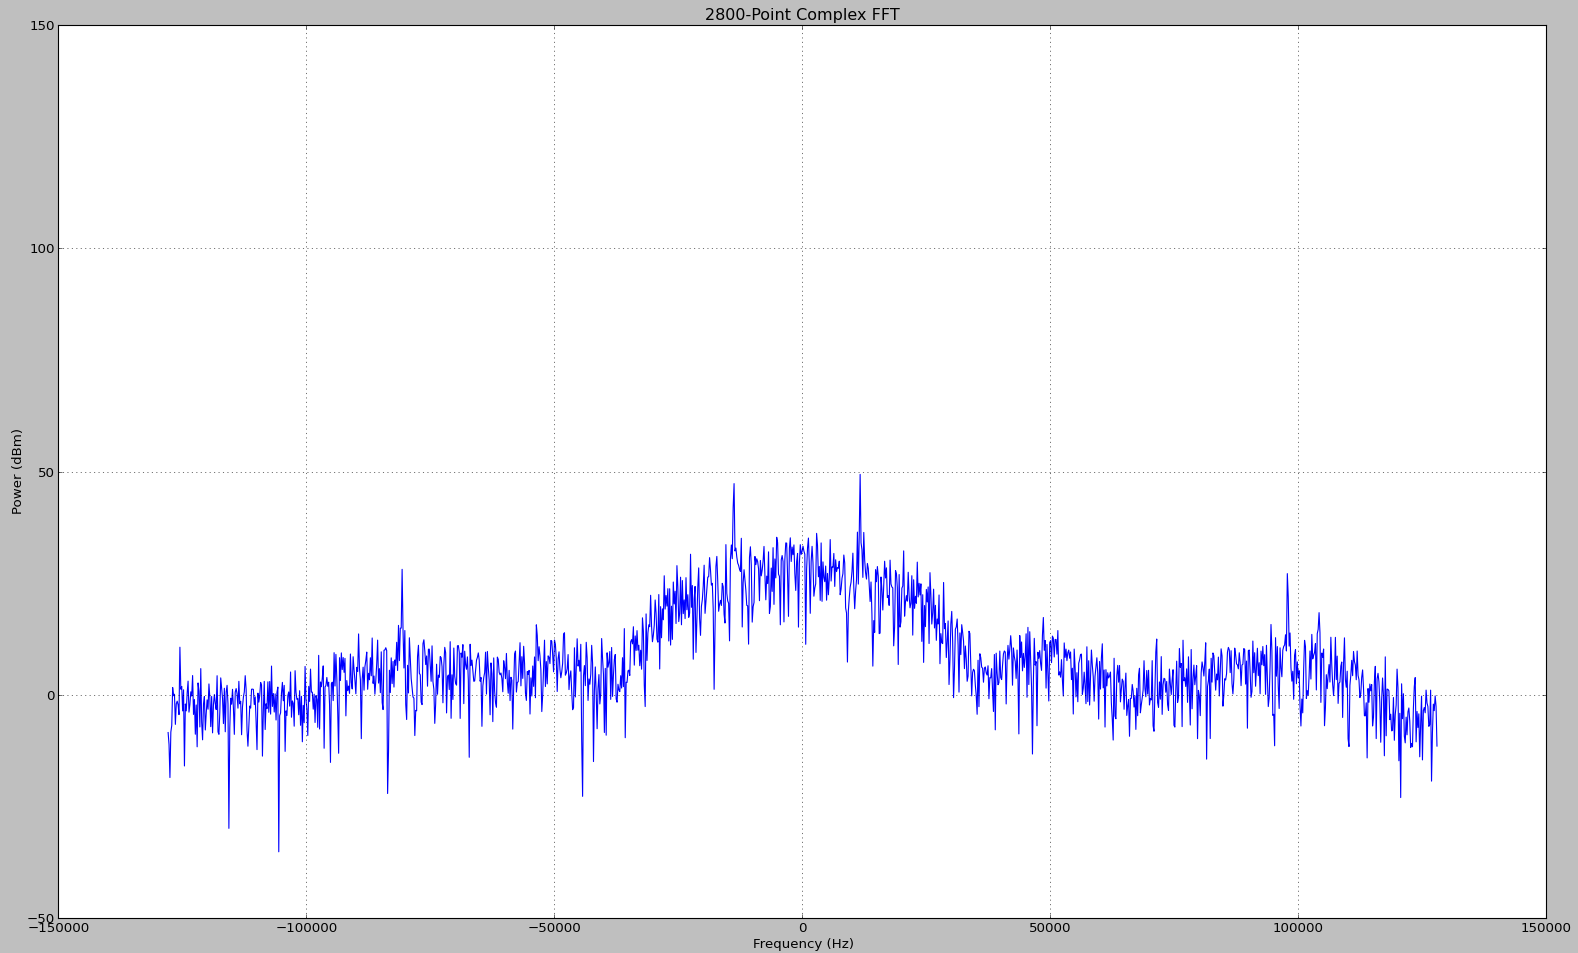
\includegraphics[scale=.2]{rx_app_fft_plot}
		\caption{Output of RX app}
		\label{fig:rx_app_fft_plot}
	\end{figure}
\noindent Alternatively, the shortened file can be plotted which will ignore optionally unwanted startup data:\par\medskip
\noindent\texttt{python ./scripts/plotAndFftAndTime.py odata/rx\_app\_shortened.out complex 18000 256000 16352}\par\medskip
\noindent The default sample rate for the GNUradio block diagram is 512 kS/s. It is recommended that when using RX app with this input signal that a sample rate close to 512 kS/s be used. Higher sample rates are still valid, but may produce plots that look drastically different than those shown here.\par\medskip
\noindent Timestamps are embedded, optionally, in the output file, and in addition to plotting, the script parses out and prints the timestamps. An example output gathered using the syntax above:\par\medskip
\scriptsize\noindent\texttt{Timestamp at index: 000000000 :  1.0728292 Seconds: 0x1 Fraction: 0x12a4eec4  \\
Timestamp at index: 000008180 :  1.0887978 Seconds: 0x1 Fraction: 0x16bb73ba ('Delta: 0.0159686', 'Expected:, 0.0159688')\\
Timestamp at index: 000016360 :  1.1047664 Seconds: 0x1 Fraction: 0x1ad1f906 ('Delta: 0.0159686', 'Expected:, 0.0159688')}\par\medskip
\noindent\small A small discrepancy (+/- 10) between Delta and Expected is typical. The difference is an artifact of the resolution of the fractional part of the timestamp applied in the timestamper HDL component. More information can be found in the timestamper component datasheet.\par\medskip
\par\medskip

\subsection{Using a RF Signal Generator}
\noindent An arbitrary RF signal generator can be used with RX app instead of the Ettus N210. \\

\noindent\textbf{Hardware Setup}
\begin{itemize}
  \item Signal generator is set to 2400.8 MHz with an amplitude of -40 dBm.
  \item Signal generator is connected to the E310 TRXA SMA.
\end{itemize}
\textbf{\\Example 1 - Execution (remote system)}\\
An example run with an IF tune freq of 0.1 MHz would be as follows.
\lstset{language=bash, backgroundcolor=\color{lightgray}, columns=flexible, breaklines=true, prebreak=\textbackslash, basicstyle=\ttfamily, showstringspaces=false,upquote=true, aboveskip=\baselineskip, belowskip=\baselineskip}
\begin{lstlisting}
SAMP_RATE_MHZ=2.5
RF_TUNE_FREQ_MHZ=2400
IF_TUNE_FREQ_MHZ=0.1
./<target>/rx_app $RF_TUNE_FREQ_MHZ $SAMP_RATE_MHZ -1 24 2.5 -1 $IF_TUNE_FREQ_MHZ 1 1 e3xx TRXA
\end{lstlisting}
\noindent\textbf{Example 1 - Verification (development system)}\\
Verify that the signal generator tone exists at 700,000 Hz in the plotted baseband signal FFT (calculated as signal generator frequency - RF tune frequency - IF tune frequency = 2400.8 MHz - 2400 MHz - 0.1 MHz = 700,000 Hz).
\begin{lstlisting}
SAMP_RATE_HZ=2500000
python ./scripts/plotAndFftAndTime.py odata/rx_app_shortened.out complex 65536 $SAMP_RATE_HZ 16352 &
\end{lstlisting}
        \begin{figure}[H]
        \begin{minipage}{.5\textwidth}
                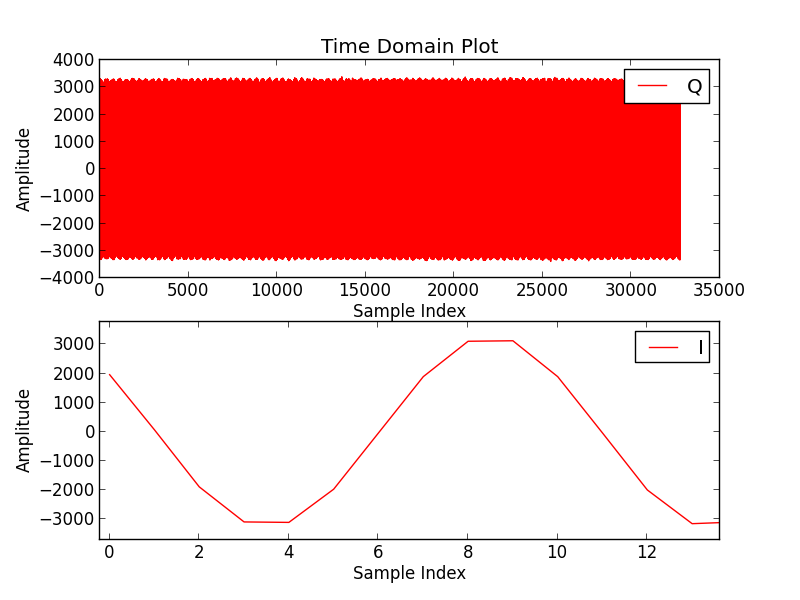
\includegraphics[width=7cm,height=5.5cm,keepaspectratio]{rx_app_sig_gen_time_domain}
                \label{fig:rx_app_sig_gen_time_domain}
        \end{minipage}%
        \begin{minipage}{.5\textwidth}
                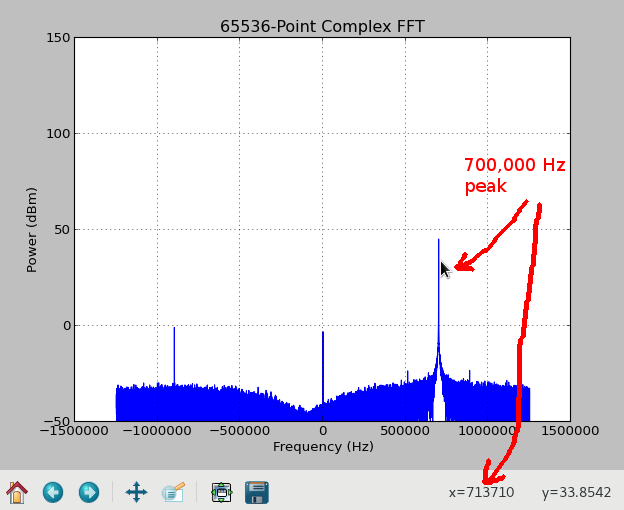
\includegraphics[width=7cm,height=5.5cm,keepaspectratio]{rx_app_sig_gen_fft}
        \end{minipage}
                \caption{Output of RX app}
                \label{fig:rx_app_sig_gen_fft}
        \end{figure}
\pagebreak
\textbf{\\Example 2 - Execution (remote system)}\\
An example run with an IF tune freq of 0 MHz would be as follows.
\begin{lstlisting}
SAMP_RATE_MHZ=2.5
RF_TUNE_FREQ_MHZ=2400
IF_TUNE_FREQ_MHZ=0
./<target>/rx_app $RF_TUNE_FREQ_MHZ $SAMP_RATE_MHZ -1 24 2.5 -1 $IF_TUNE_FREQ_MHZ 1 1 e3xx TRXA
\end{lstlisting}
\noindent\textbf{Example 2 - Verification (development system)}\\
Verify that the signal generator tone exists at 800,000 Hz in the plotted baseband signal FFT (calculated as signal generator frequency - RF tune frequency - IF tune frequency = 2400.8 MHz - 2400 MHz - 0 MHz = 800,000 Hz).
\begin{lstlisting}
SAMP_RATE_HZ=2500000
python ./scripts/plotAndFftAndTime.py odata/rx_app_shortened.out complex 65536 $SAMP_RATE_HZ 16352 &
\end{lstlisting}
        \begin{figure}[H]
        \begin{minipage}{.5\textwidth}
                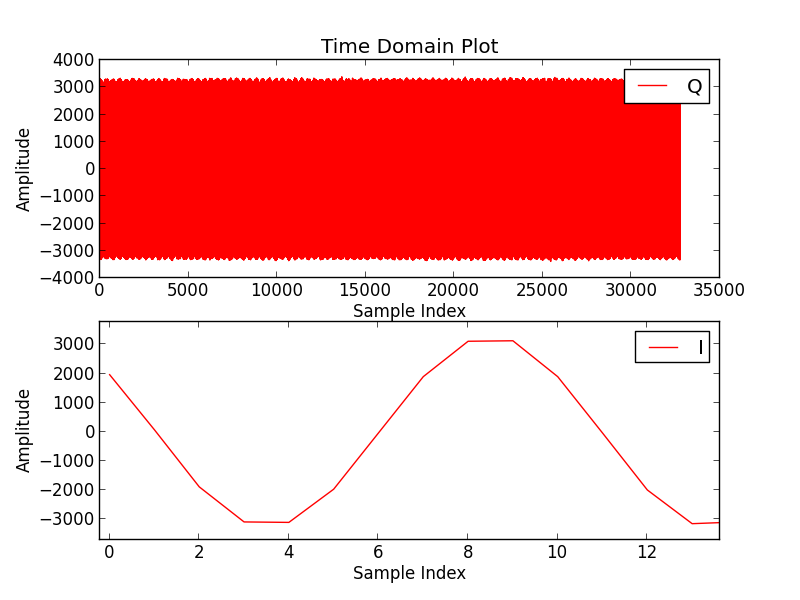
\includegraphics[width=7cm,height=5.5cm,keepaspectratio]{rx_app_sig_gen_time_domain}
                \label{fig:rx_app_sig_gen_time_domain}
        \end{minipage}%
        \begin{minipage}{.5\textwidth}
                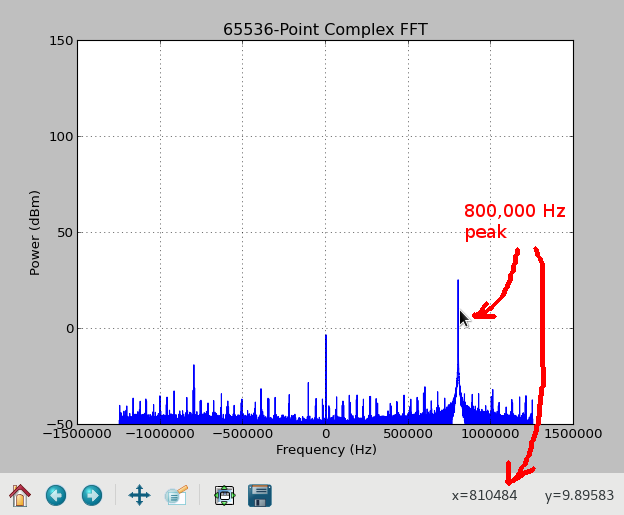
\includegraphics[width=7cm,height=5.5cm,keepaspectratio]{rx_app_sig_gen_fft_800k}
        \end{minipage}
                \caption{Output of RX app}
                \label{fig:rx_app_sig_gen_fft}
        \end{figure}
\subsection{Known Issues}
\noindent
\begin{itemize}
  \item If the path \path{/var/volatile} does not exist or requires root permission to write to, you will need to modify the ACI and the application XML to use a different directory for writing data. This involves simply finding and replacing \path{/var/volatile} with a different directory in the \path{.cxx} and \path{.xml} files. Failing to make this change when necessary may result in a segmentation fault error at application runtime.
\end{itemize}
% AV-3179
\section{Appendix A: Worker Parameters}
\begin{minipage}[t]{.5\textwidth}
	\textbf{E310}
	\begin{itemize}
		\item cic\_dec.hdl
			\subitem N = 3
			\subitem M = 1
			\subitem R = 8
			\subitem DIN\_WIDTH = 16
			\subitem ACC\_WIDTH = 25
			\subitem DOUT\_WIDTH = 16
		\item complex\_mixer.hdl
			\subitem NCO\_DATA\_WIDTH\_p = 12
			\subitem INPUT\_DATA\_WIDTH\_p = 12
			\subitem CORDIC\_STAGES\_p = 16
			\subitem PEAK\_MONITOR\_p = true
		\item iq\_imbalance\_fixer.hdl
			\subitem DATA\_WIDTH\_p = 16
			\subitem ACC\_PREC\_p = 34
			\subitem PEAK\_MONITOR\_p = true
		\item dc\_offset\_filter.hdl
			\subitem DATA\_WIDTH\_p = 16
			\subitem PEAK\_MONITOR\_p = true
		\item e3xx\_i2c.hdl
			\subitem CP\_CLK\_FREQ\_p = 100e6
			\subitem FMC\_GA1 = 0
			\subitem FMC\_GA0 = 0
		\item ad9361\_spi.hdl
			\subitem CP\_CLK\_FREQ\_HZ\_p = 100e6
		\item ad9361\_data\_sub.hdl
			\subitem LVDS\_p = false
			\subitem HALF\_DUPLEX\_p = false
			\subitem SINGLE\_PORT\_p = true
			\subitem SWAP\_PORTS\_p = false
			\subitem DATA\_CLK\_Delay = 11
			\subitem RX\_Data\_Delay = 0
			\subitem FB\_CLK\_DELAY = 12
			\subitem TX\_DATA\_DELAY = 0
		\item ad9361\_adc\_sub
			\subitem LVDS\_p = false
			\subitem HALF\_DUPLEX\_p = false
			\subitem SINGLE\_PORT\_p = true
		\item ad9361\_dac\_sub
			\subitem LVDS\_p = false
			\subitem HALF\_DUPLEX\_p = false
			\subitem SINGLE\_PORT\_p = true
	\end{itemize}
\end{minipage} \newpage
\section{Appendix B: Artifacts}
\subsection{E310}
	\begin{itemize}
	\item dc\_offset\_iq\_imbalance\_mixer\_cic\_dec\_timestamper\_e3xx\_cfg\_1rx\_0tx\_mode\_2\_cmos\_cnt\_1rx\_0tx\_thruasm\_mode\_2\_cmos\_e3xx.bitz
	\item target-xilinx13\_4/file\_write\_s.so
	\item target-xilinx13\_4/e3xx\_rx\_s.so
	\item target-xilinx13\_4/e3xx\_mimo\_xcvr\_filter\_proxy\_s.so
	\item target-xilinx13\_4/ad9361\_config\_proxy\_s.so
	\end{itemize}
\end{document}
